%!TEX TS-program = xelatex
%!TEX encoding = UTF-8 Unicode

\documentclass[a4paper]{article}

\usepackage{xltxtra}
\usepackage{amsfonts}
\usepackage{polyglossia}
\usepackage{fancyhdr}
\usepackage{geometry}
\usepackage{dsfont}
\usepackage{amsmath}
\usepackage{amsthm}
\usepackage{amssymb}
\usepackage{physics}
\usepackage{mathtools}
\usepackage{float}
\usepackage[shortlabels]{enumitem}

\geometry{a4paper,left=15mm,right=15mm,top=20mm,bottom=20mm}
\pagestyle{fancy}
\lhead{Devon Morris}
\chead{Dynamics}
\rhead{\today}
\cfoot{\thepage}

\setlength{\headheight}{23pt}
\setlength{\parindent}{0.0in}
\setlength{\parskip}{0.0in}

\newtheorem*{prop}{Proposition}
\newtheorem*{defn}{Definition}
\newtheorem*{thm}{Theorem}
\newtheorem*{cor}{Corollary}
\newtheorem*{lem}{Lemma}
\newtheorem*{rem}{Remark}

\DeclarePairedDelimiterX{\inn}[2]{\langle}{\rangle}{#1, #2}

\begin{document}
\section*{Final Project: Apollo Spacecraft Attitude Dynamics}%

\subsection*{Task A:}%
Let $\hat{i}$, $\hat{j}$, $\hat{k}$ be the unit vectors of the $A$ frame.
\begin{enumerate}[a.]
  \item General Case:
    The location of the center of mass is
    \[
      r_{G/A} = 23.6177 \hat{i} + 0.0961 \hat{j} + -0.0087 \hat{k}\ m
    \]
    which gives us the inertia matrix of
    \[
      \begin{aligned}
        [I_{G/A}] &= [I_{SM/A}] + [I_{CM/A}] + [I_{PROP/A}] \\
                  &= 
                  \begin{bmatrix}
                    I_{xx} & -I_{xy} & -I_{xz} \\
                    -I_{xy} & I_{yy} & -I_{yz} \\
                    -I_{xz} & -I_{yz} & I_{zz}
                  \end{bmatrix} \\
            &=
            \begin{bmatrix}
              40823.073 &  1537.807 & -3179.297 \\
              1537.807 & 90593.489 & 128.577 \\
              -3179.297 & 128.577 & 98742.852
            \end{bmatrix}
      \end{aligned}
    \]
  \item Simplified Case:
    The location of the center of mass is
    \[
      r_{G/A} = 23.6177 \hat{i}\ m
    \]
    which gives us the inertia matrix of
    \[
      [I_{G/A}] = 
      \begin{bmatrix}
        40481.983 & 0 & 0 \\
        0 & 90358.316 & 0 \\
        0 & 0 & 98636.935
      \end{bmatrix}
    \]
\end{enumerate}

\subsection*{Task B:}%
First we have that the euler angle rates and angular velocities are related by
\[
  \begin{aligned}
    \omega_x &= - \dot{\psi} s_{\theta} + \dot{\phi} \\
    \omega_y &= \dot{\psi} c_{\theta}s_{\phi} + \dot{\theta} c_{\phi} \\
    \omega_z &= \dot{\psi}c_{\theta}c_{\phi} - \dot{\theta}s_{\phi}
  \end{aligned}
\]
Using these in the general rotational equations (and using Matlab's symbolic toolbox) gives the six equations of motion
\[
  \begin{aligned}
    \dv{t} \left( \phi \right) =& \dot{\phi} \\ 
    \dv{t} \left( \theta \right) =& \dot{\theta} \\
    \dv{t} \left( \psi \right) =& \dot{\psi} \\
    M_x =& 
\left(-I_{xx}\,s_\theta-I_{xz}\,c_\phi\,c_\theta-I_{xy}\,c_\theta\,s_\phi\right)\,\ddot{\psi}+I_{xx}\,\ddot{\phi}+\left(I_{xz}\,s_\phi-I_{xy}\,c_\phi\right)\,\ddot{\theta} \\ 
         &+\left(I_{yz}\,{c_\phi}^2\,{c_\theta}^2-I_{yz}\,{c_\theta}^2\,{s_\phi}^2-I_{xy}\,c_\phi\,c_\theta\,s_\theta+I_{xz}\,c_\theta\,s_\phi\,s_\theta-I_{yy}\,c_\phi\,{c_\theta}^2\,s_\phi+I_{zz}\,c_\phi\,{c_\theta}^2\,s_\phi\right)\,{\dot{\psi}}^2 \\
         &+\left(2\,I_{xz}\,c_\phi\,s_\theta-I_{xx}\,c_\theta+2\,I_{xy}\,s_\phi\,s_\theta-I_{yy}\,{c_\phi}^2\,c_\theta+I_{zz}\,{c_\phi}^2\,c_\theta+I_{yy}\,c_\theta\,{s_\phi}^2-I_{zz}\,c_\theta\,{s_\phi}^2-4\,I_{yz}\,c_\phi\,c_\theta\,s_\phi\right)\,\dot{\psi}\,\dot{\theta} \\
         &+\left(I_{yz}\,{s_\phi}^2-I_{yz}\,{c_\phi}^2+I_{yy}\,c_\phi\,s_\phi-I_{zz}\,c_\phi\,s_\phi\right)\,{\dot{\theta}}^2 \\
    M_y =&
\left(I_{xy}\,s_\theta-I_{yz}\,c_\phi\,c_\theta+I_{yy}\,c_\theta\,s_\phi\right)\,\ddot{\psi}+\left(-I_{xy}\right)\,\ddot{\phi}+\left(I_{yy}\,c_\phi+I_{yz}\,s_\phi\right)\,\ddot{\theta} \\
         &+\left(I_{xz}\,{s_\theta}^2-I_{xz}\,{c_\phi}^2\,{c_\theta}^2-I_{xx}\,c_\phi\,c_\theta\,s_\theta+I_{zz}\,c_\phi\,c_\theta\,s_\theta-I_{yz}\,c_\theta\,s_\phi\,s_\theta-I_{xy}\,c_\phi\,{c_\theta}^2\,s_\phi\right)\,{\dot{\psi}}^2 \\
         &+\left(I_{xx}\,c_\phi\,c_\theta-2\,I_{xz}\,s_\theta+I_{yy}\,c_\phi\,c_\theta-I_{zz}\,c_\phi\,c_\theta+2\,I_{yz}\,c_\theta\,s_\phi\right)\,\dot{\psi}\,\dot{\phi} \\
         &+\left(I_{xy}\,c_\theta+I_{xx}\,s_\phi\,s_\theta-I_{yy}\,s_\phi\,s_\theta-I_{zz}\,s_\phi\,s_\theta-I_{xy}\,{c_\phi}^2\,c_\theta+I_{xy}\,c_\theta\,{s_\phi}^2+2\,I_{xz}\,c_\phi\,c_\theta\,s_\phi\right)\,\dot{\psi}\,\dot{\theta} \\
         &+I_{xz}\,{\dot{\phi}}^2+\left(2\,I_{yz}\,c_\phi-I_{xx}\,s_\phi-I_{yy}\,s_\phi+I_{zz}\,s_\phi\right)\,\dot{\phi}\,\dot{\theta}+\left(I_{xy}\,c_\phi\,s_\phi-I_{xz}\,{s_\phi}^2\right)\,{\dot{\theta}}^2 \\
    M_z =&
\left(I_{xz}\,s_\theta+I_{zz}\,c_\phi\,c_\theta-I_{yz}\,c_\theta\,s_\phi\right)\,\ddot{\psi}+\left(-I_{xz}\right)\,\ddot{\phi}+\left(-I_{yz}\,c_\phi-I_{zz}\,s_\phi\right)\,\ddot{\theta} \\
         &+\left(I_{xy}\,{c_\theta}^2\,{s_\phi}^2-I_{xy}\,{s_\theta}^2+I_{yz}\,c_\phi\,c_\theta\,s_\theta+I_{xx}\,c_\theta\,s_\phi\,s_\theta-I_{yy}\,c_\theta\,s_\phi\,s_\theta+I_{xz}\,c_\phi\,{c_\theta}^2\,s_\phi\right)\,{\dot{\psi}}^2 \\
         &+\left(2\,I_{xy}\,s_\theta-2\,I_{yz}\,c_\phi\,c_\theta-I_{xx}\,c_\theta\,s_\phi+I_{yy}\,c_\theta\,s_\phi-I_{zz}\,c_\theta\,s_\phi\right)\,\dot{\psi}\,\dot{\phi} \\
         &+\left(I_{xz}\,c_\theta+I_{xx}\,c_\phi\,s_\theta-I_{yy}\,c_\phi\,s_\theta-I_{zz}\,c_\phi\,s_\theta+I_{xz}\,{c_\phi}^2\,c_\theta-I_{xz}\,c_\theta\,{s_\phi}^2+2\,I_{xy}\,c_\phi\,c_\theta\,s_\phi\right)\,\dot{\psi}\,\dot{\theta} \\
         &-I_{xy}\,{\dot{\phi}}^2+\left(I_{yy}\,c_\phi-I_{xx}\,c_\phi-I_{zz}\,c_\phi+2\,I_{yz}\,s_\phi\right)\,\dot{\phi}\,\dot{\theta}+\left(I_{xy}\,{c_\phi}^2-I_{xz}\,c_\phi\,s_\phi\right)\,{\dot{\theta}}^2
  \end{aligned}
\]
\subsection*{Task C:}%
\begin{enumerate}[a.]
  \item  See attached \texttt{morris.m}
  \item  Here are the plots of the general case
    \begin{figure}[H]
    \begin{center}
      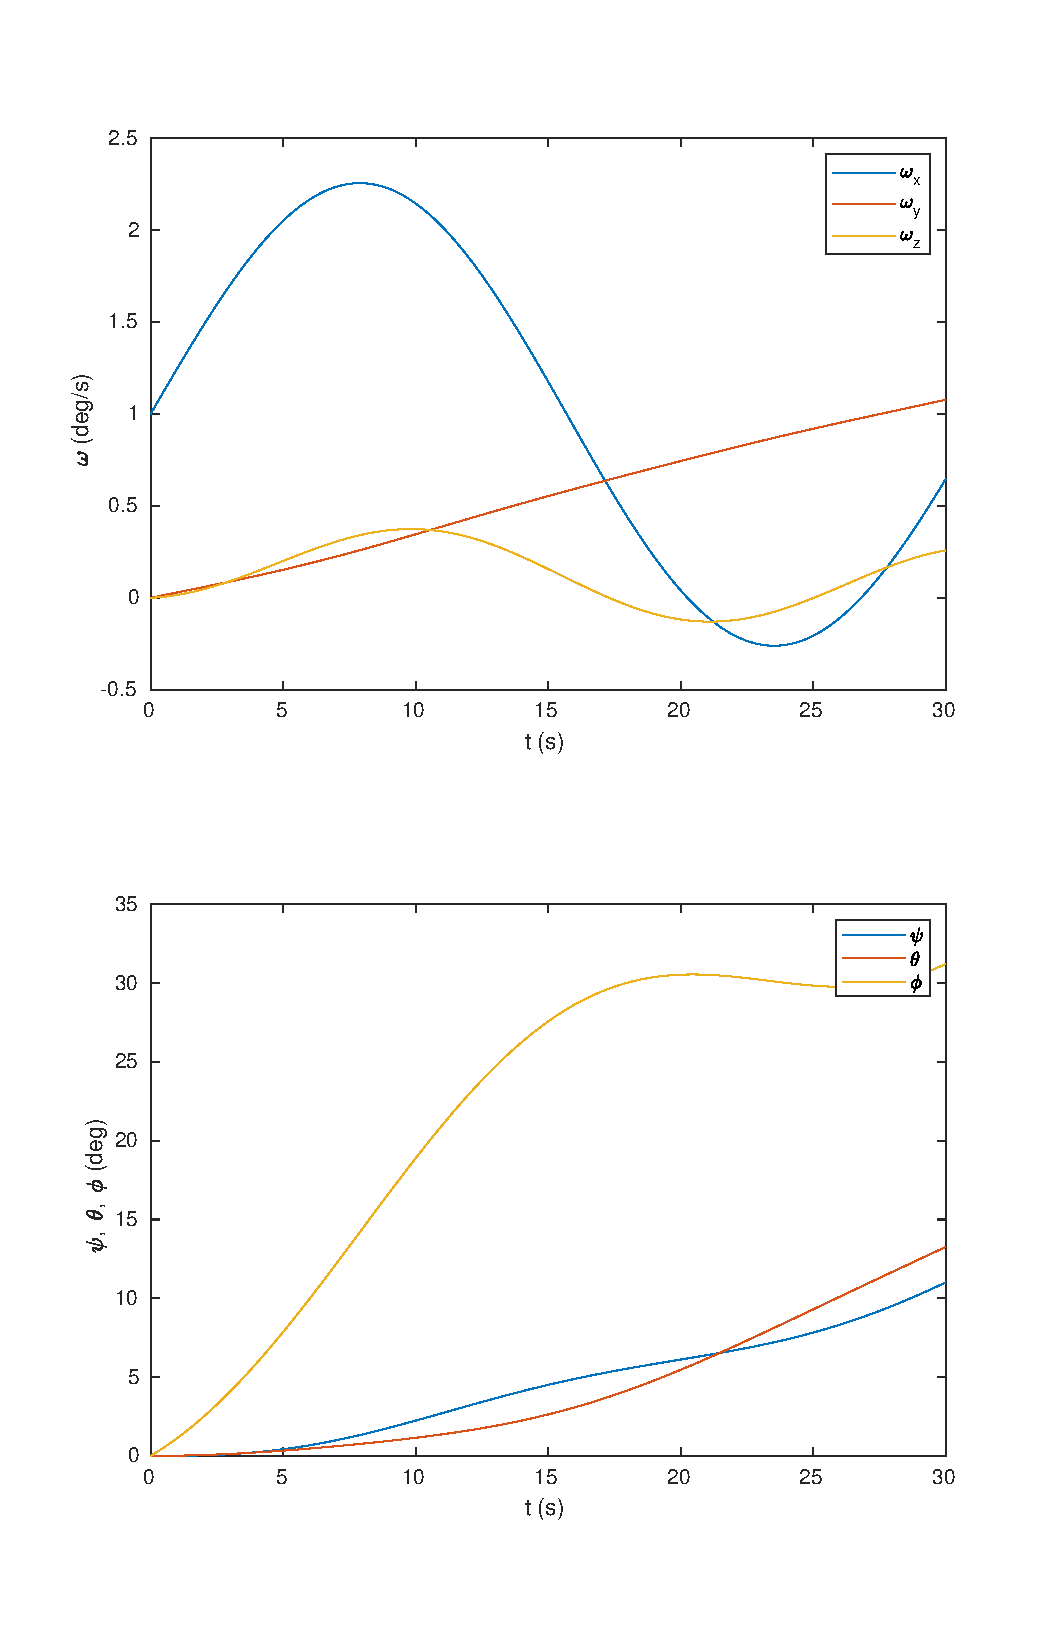
\includegraphics[scale=0.7]{task_c.eps}
    \end{center}
    \caption{Simulation of CSM attitude (General)}
    \label{fig:task_c}
    \end{figure}

    Here is a table of maximum and minimum values in the general case
    \begin{table}[H]
      \centering
      \begin{tabular}{lcccccc}
        & $\omega_x$ & $\omega_y$ & $\omega_z$ & $\psi$ & $\theta$ & $\phi$ \\
        $\max$ &  2.2554 & 1.0744 & 0.3740 & 11.0113 & 13.2593 & 31.2242\\
        $\min$ & -0.2605 & 0.0000 & -0.1293 & 0.0000 & 0.0000 & 0.0000 \\
      \end{tabular}
      \caption{Table of max and min values shown in degrees and degrees per second (General)}
    \end{table}

    \begin{figure}[H]
    \begin{center}
      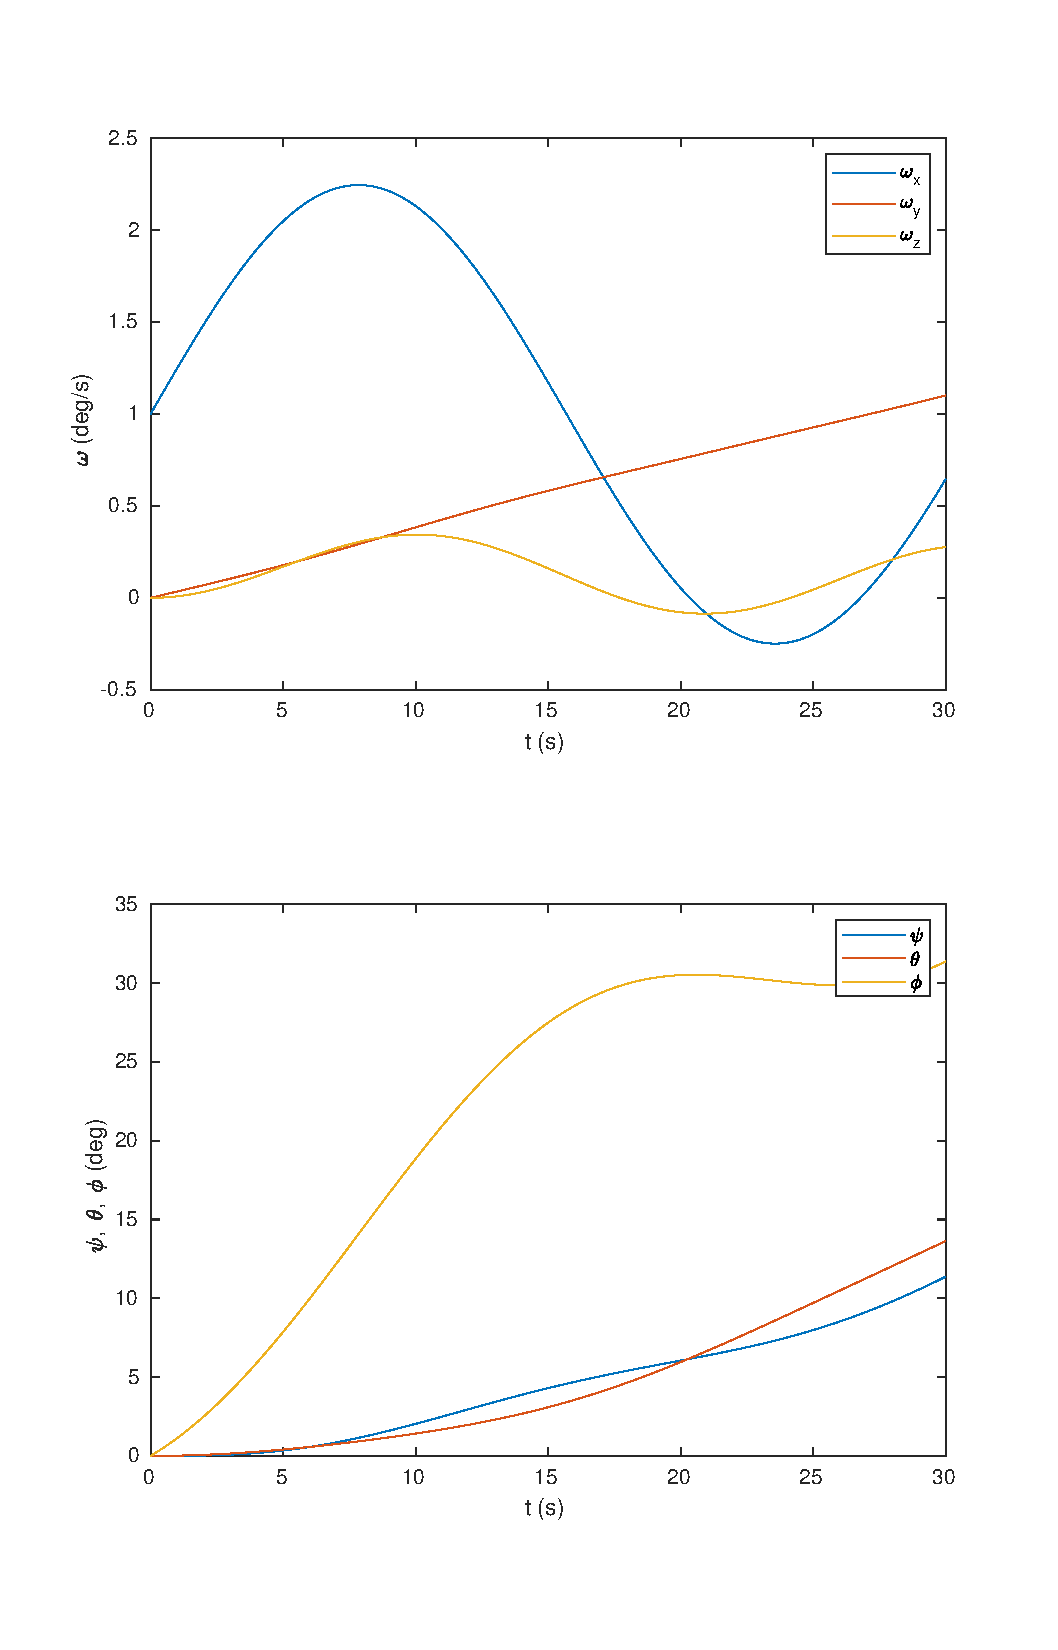
\includegraphics[scale=0.7]{task_c_simplified.eps}
    \end{center}
    \caption{Simulation of CSM attitude (Simplified)}
    \label{fig:task_c_simplified}
    \end{figure}

    Here is a table of maximum and minimum values in the simplified case
    \begin{table}[H]
      \centering
      \begin{tabular}{lcccccc}
        & $\omega_x$ & $\omega_y$ & $\omega_z$ & $\psi$ & $\theta$ & $\phi$ \\
        $\max$ &  2.2448 & 1.1006 & 0.3439 & 11.3695 & 13.6357 & 31.3756 \\
        $\min$ & -0.2489 & 0.0000 & -0.0859 & 0.0000 & 0.0000 & 0.0000 \\
      \end{tabular}
      \caption{Table of max and min values shown in degrees and degrees per second (Simplified)}
    \end{table}
  \item I calculated that the torques need to be
    \[
      \begin{aligned}
        M_x &= 0.000000\ Nm \\
        M_y &= 0.968469\ Nm\\
        M_z &= 0.468443\ Nm
      \end{aligned}
    \]
    When these torques are applied the following response is observed.
    \begin{figure}[H]
    \begin{center}
      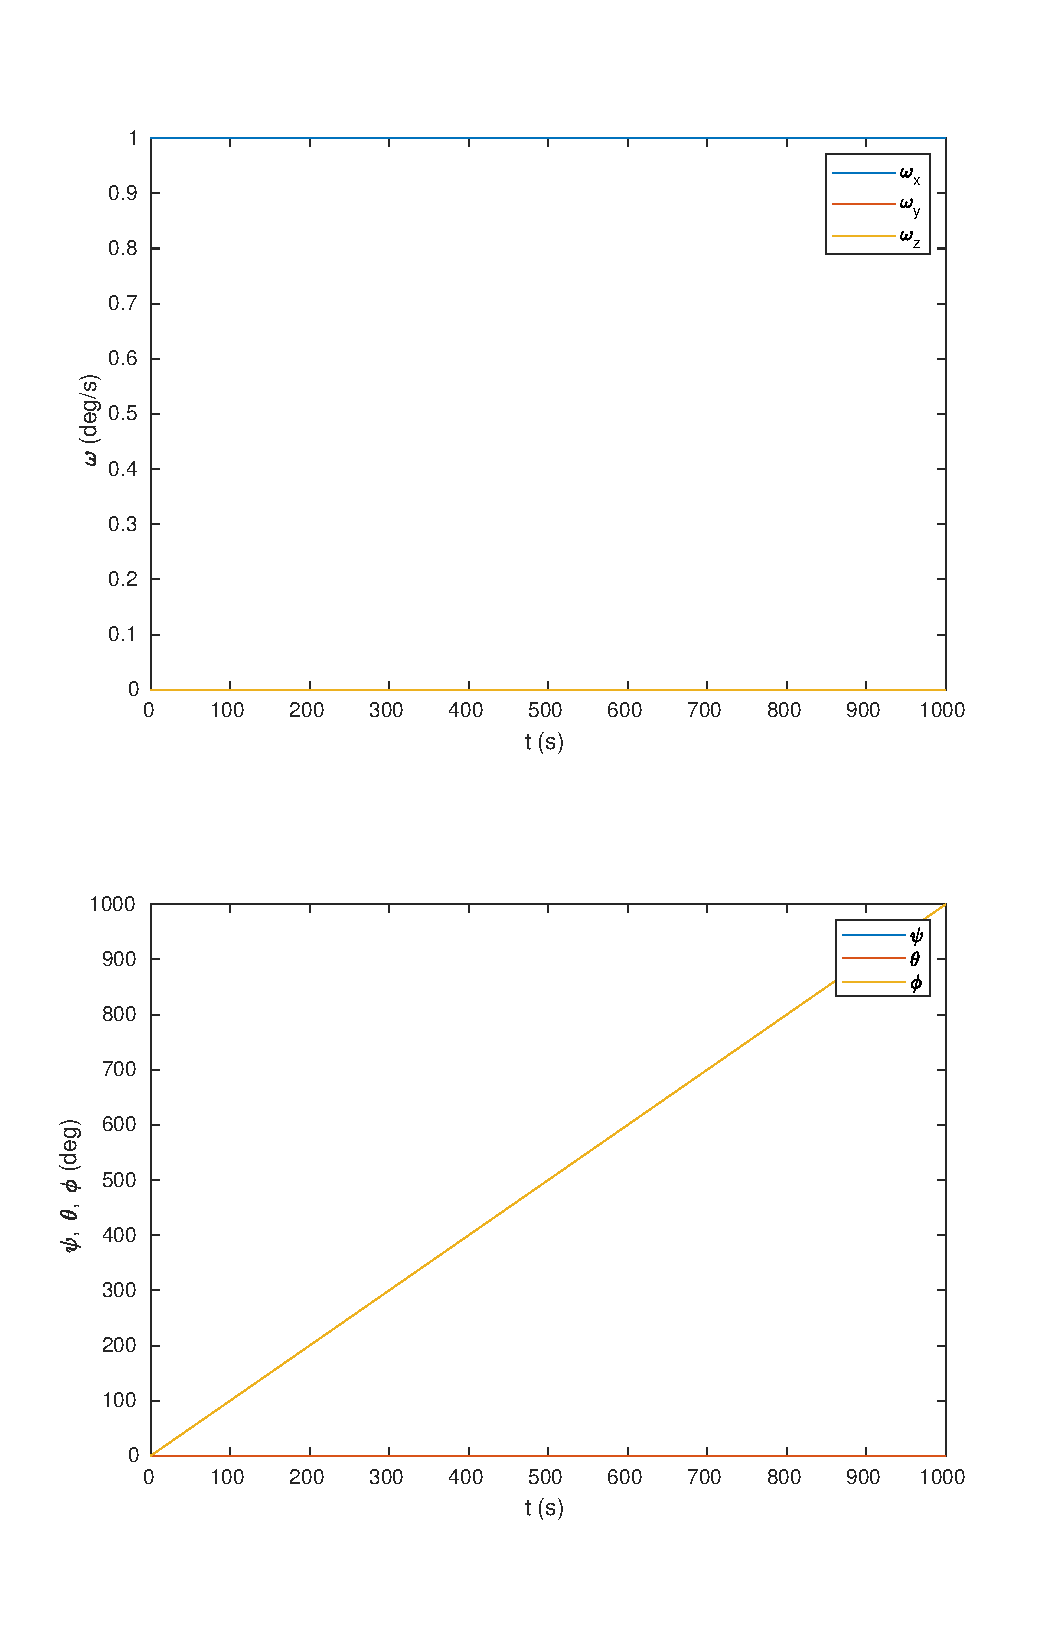
\includegraphics[scale=0.7]{task_c_torques.eps}
    \end{center}
    \caption{Simulation of CSM attitude with constant torques}
    \label{fig:task_c_torques}
    \end{figure}

    When no torques are applied the following response is observed
    \begin{figure}[H]
    \begin{center}
      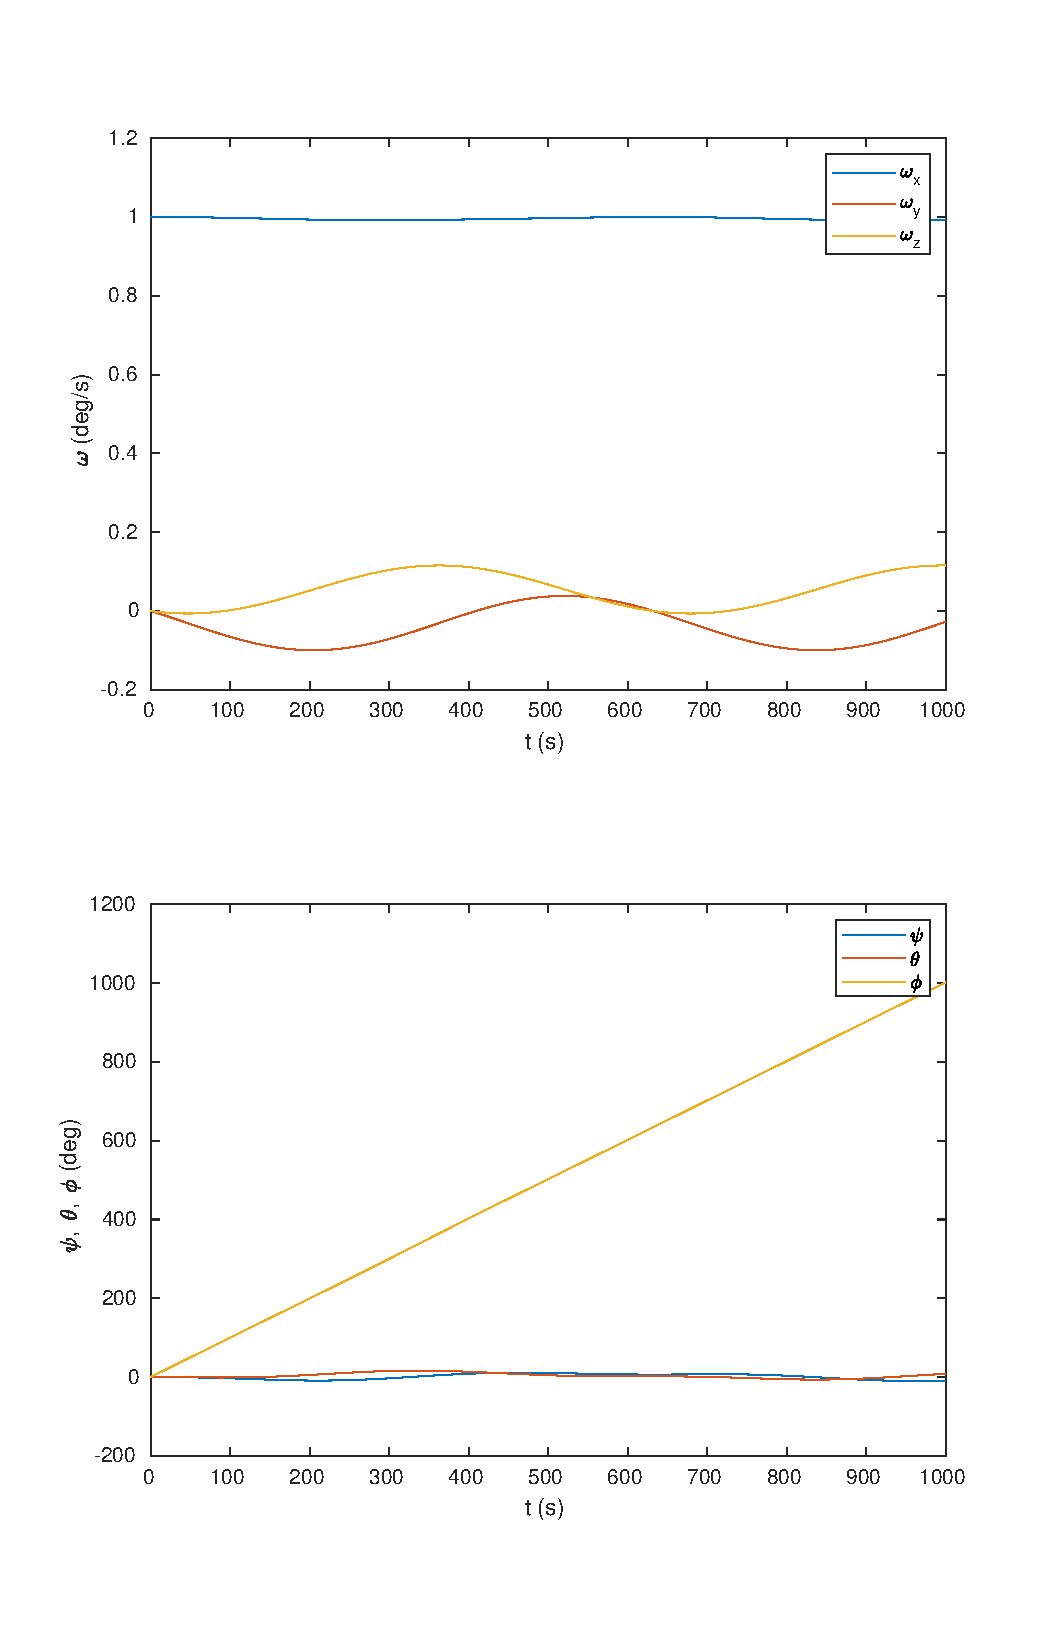
\includegraphics[scale=0.7]{task_c_no_torques.eps}
    \end{center}
    \caption{Simulation of CSM attitude with no applied torques}
    \label{fig:task_c_no_torques}
    \end{figure}


\end{enumerate}

\end{document}
